 \documentclass{report}
 
\usepackage[utf8]{inputenc} 
\usepackage[T1]{fontenc}      
\usepackage[top=3.5cm, bottom=3cm, left=3.0cm, right=4.0cm]{geometry}
\usepackage{graphicx}
\usepackage{wrapfig}
\usepackage{amsmath}
\graphicspath{{figures/}{../figures}}

\begin{document}

\section*{Exercice 1}

\subsubsection*{Transfert d'une fusée d'une orbite terrestre à l'orbite lunaire}

On considère une fusée placée sur une orbite terrestre basse (altitude de 2000km), de masse à vide $M_0=10$t et remplie d'un mélange carburant-comburant appelé \textit{ergols} de masse initiale $m_0$. A $t=0$, la fusée allume ses propulseurs pour se diriger vers l'orbite lunaire ou martienne. La combustion d'ergol éjecte des gaz à une vitesse $v_e$ par rapport à celle de la fusée et à un débit massique $D_m$, qui reste constant tout au long de la combustion. Après la combustion totale des ergols, la fusée acquiert un supplément de vitesse $\Delta V$.

\begin{itemize}

	\item[$\clubsuit$] Trouver une relation, dite \textit{équation de Tsiolkovski} entre $\Delta V$ et la proportion $m_0/(m_0+M_0)$, cad la proportion entre la masse initiale d'ergols et la masse totale de la fusée. 
	
	\item[$\clubsuit$] Pour atteindre l'orbite lunaire, il faut d'abord acquérir un supplément de vitesse égal à $\Delta V=2,8$km.s$^{-1}$ puis ralentir de la même quantité de vitesse (la fusée peut soit accélérer soit ralentir grâce à son système de propulsion). Quelle masse d'ergols faut-il prévoir ?
	
\end{itemize}

\subsubsection*{Condition de décollage d'une fusée}

On s'intéresse désormais au décollage de la fusée depuis la terre ferme. La fusée a toujours les même caractéristiques, elle est désormais soumise au champs de pesanteur $\vec{g}$, supposé uniforme. La résistance de l'air est négligée. 

\begin{itemize}

\item[$\clubsuit$] Montrer que la fusée ne peut décoller que si $D_m$ est supérieur à une certaine valeur.
\item[$\clubsuit$] En supposant que $D_m$ est suffisamment important pour permettre le décollage, calculez la vitesse finale de la fusée une fois que tous les ergols ont été consommés, ainsi que l'altitude atteinte.

\end{itemize}

\newpage

\section*{Exercice 2}

Une turbine de barrage est un cylindre de rayon $a$ avec des pâles à ses extrémités, entraînées par un jet d'eau. Elle tourne autour de son axe à la vitesse angulaire $\omega$. Un jet incident, d'épaisseur négligeable, arrive avec un débit massique $D_m$ sur la turbine avec une vitesse $\vec{v_1}$ et ressort avec une vitesse $\vec{v_2}$, toutes deux tangentielles à la turbine.

\begin{center}
	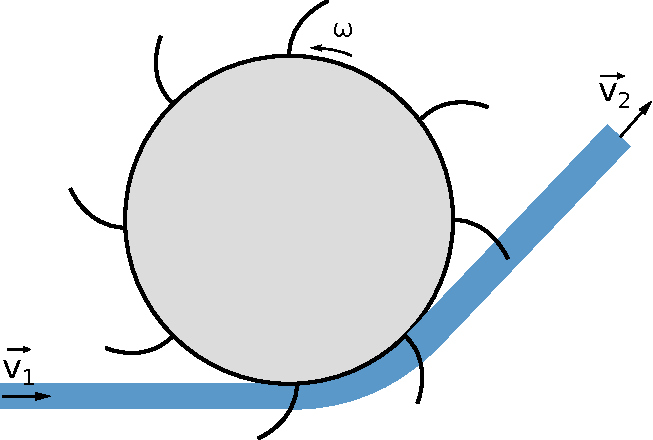
\includegraphics[scale=0.5]{meca_flu7.pdf}
\end{center}

La turbine a un moment d'inertie $J$ autour de son axe. Elle est ralentie par un générateur et des frottements qui opposent un couple de résistance $\Gamma$. On négligera l'action de la pesanteur.

\begin{itemize}

	\item[$\spadesuit$] A l'aide de bilans, trouver deux relations entre $\omega$,  $\vec{v_1}$,  $\vec{v_2}$ et les données de l'énoncé.
	
	\item[$\spadesuit$] Trouver l'expression de $\omega_P$, la vitesse de rotation en régime permanent. 
	
	\item[$\spadesuit$] La vitesse $v_1$ et $D_m$ étant données, quelle est la valeur de $\Gamma$ pour laquelle la puissance $P$ transmise à la turbine est maximale ? Commenter le résultat.
	
	\item[$\spadesuit$] On choisit $\Gamma$ de sorte à ce que $P$ soit maximale. La turbine est à l'arrêt à $t=0$, déterminer $\omega$ au cours du temps. Quelle est le temps caractéristique d'établissement permanent ?
	
	\item[$\spadesuit$] On suppose que la turbine est en bas d'un barrage de 100m de haut, obstruant le lit d'une rivière d'un débit de 100m$^3$/s. Quelle est la vitesse $v_1$ de l'eau à la sortie du barrage ? En supposant que le rendement de conversion de la puissance mécanique de la turbine à un alternateur est de 90\%, quelle puissance électrique peut-on extraire d'une telle rivière ? Retrouver ce calcul à l'aide d'une autre méthode.
	
	\item[$\spadesuit$] En moyenne, il pleut environ une hauteur 1000mm d'eau par an sur le territoire Français, qui fait 547 000km$^2$. Seulement 40\% de cette quantité d'eau s'écoule dans les fleuves et rivière, le reste s'écoule soit dans les nappes phréatiques, soit s'évapore. Sachant que l'altitude moyenne du pays est de 342m, en déduire le potentiel de production d'énergie hydroélectrique sur une année. Comparer avec la production actuelle qui est de 63TWh/an et la consommation d'énergie finale en France, qui est de 1629TWh/an.

\end{itemize}

\newpage

\section*{Exercice 3}

On s'intéresse à l'interaction entre l'air et une hélice (d'avion, d'hélicoptère ou d'éolienne). On considère le tube d'air qui va traverser la section $S$ de l'hélice. L'écoulement est supposé permanent, incompressible, parfait et on néglige les effets de la pesanteur. La pression loin de l'hélice est $P_0$. 

\begin{center}
	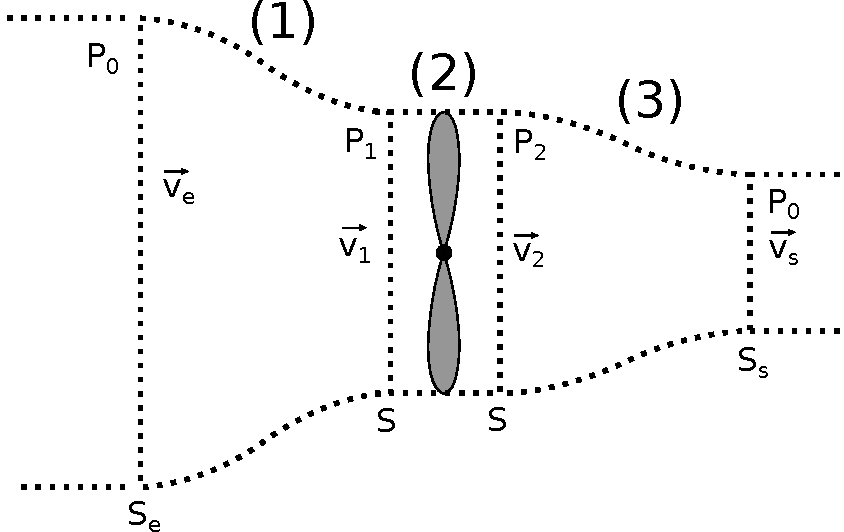
\includegraphics[scale=0.5]{meca_flu6.pdf}
\end{center}

On distingue 3 zones remarquables dans l'écoulement :
\begin{itemize}
	\item[(1) ] Cette zone correspond au passage d'un écoulement lointain de l'hélice à proche. Le tube d'air passe alors d'une section $S_e$, avec une vitesse $v_e$ et une pression $P_0$ a une section $S$, avec une vitesse $v_1$ et une pression $P_1$.
	\item[(2) ] Zone juste autour de l'hélice, l'écoulement est turbulent. Juste avant l'hélice, la vitesse est $\vec{v_1}$ et la pression $P_1$. Juste après, la vitesse est $\vec{v_2}$ et la pression $P_2$.
	\item[(3) ] Cette zone correspond au passage d'un écoulement proche de l'hélice à lointain. Le tube d'air passe alors d'une section $S$, avec une vitesse $v_2$ et une pression $P_2$ a une section $S_s$, avec une vitesse $v_s$ et une pression $P_0$.
\end{itemize}
Dans les sections (1) et (2), on suppose que l'écoulement de l'air est irrotationnel, unidimentionnel et laminaire. Les pressions et les vitesses sont donc uniformes pour une section droite donnée du tube. Toutes les vitesses seront d'ailleurs supposées dirigées uniquement suivant l'axe de rotation de l'hélice. 
On notera $\vec{F}$ la force exercée par l'hélice sur l'air et $P$ la puissance fournie au fluide.

\begin{itemize}
	\item[$\clubsuit$] Comment s'écrivent les relations de conservation du début massique ? Comparer les sections $S_e$ et $S_s$ dans le cas où l'hélice est celle d'un avion, et dans le cas où c'est celle d'une éolienne. 
	\item[$\clubsuit$] Appliquer le théorème de Bernoulli dans la zone (1) et (3). Est-ce paradoxal d'avoir $v_e\neq v_s$ alors que les pressions sont identiques et égales à $P_0$ ?
	\item[$\clubsuit$] En faisant un bilan sur une portion de fluide dans la zone (2) du tube, déterminer une expression de $F$ en fonction de $\rho$, $S$, $v_e$ et $v_s$.
	\item[$\clubsuit$] En effectuant un bilan sur une autre section de fluide, déterminer une autre expression entre $F$, $\rho$, $S$, $v_e$ et $v_s$. En déduire une relation simple entre $v_1$, $v_2$, $v_e$ et $v_s$.
	\item[$\clubsuit$] Déterminer la puissance $P$ en fonction de $\rho$, $S$, $v_e$ et $v_s$. 
	
	\item[$\clubsuit$] Démontrer la \textit{loi de Betz}, qui stipule que le rendement maximal théorique d'une éolienne est de $\eta=$16/27. Commenter.
	
\end{itemize}

\end{document}
